
\documentclass[tikz,border=5pt]{standalone}
\usetikzlibrary{arrows.meta}
\usetikzlibrary{decorations.text}
\begin{document}
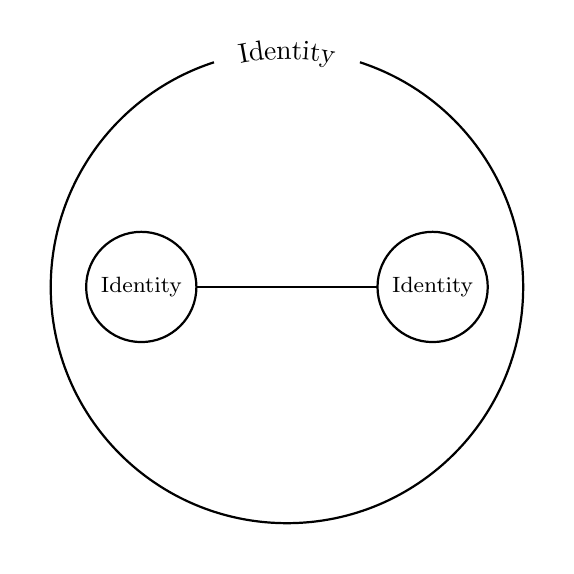
\begin{tikzpicture}[
    >=Stealth,
    every node/.style={font=\small},
    line width=0.8pt
]

\def\R{3.0}
\def\r{0.70}
\def\d{1.85}

%\draw (0,0) circle (\R);
\def\Gap{18}
% Upper left
\draw (180:\R)
      arc (180:{90+\Gap}:\R);
% Upper right
\draw ({90-\Gap}:\R)
      arc ({90-\Gap}:0:\R);
% Lower half
\draw (180:\R)
      arc (180:360:\R);
      
    
%\node[ fill=white, inner xsep=4pt, inner ysep=1pt ] at (90:\R) {Enclosure};

\path[
    decorate,
    decoration={
        text along path,
        text={Identity},
        text align=center,
        raise=-3pt
   }
]
(315:\R) arc (315:-135:\R);


\draw (-\d,0) circle (\r);
\draw ( \d,0) circle (\r);

\node[font=\footnotesize] at (-\d,0) {Identity};
\node[font=\footnotesize] at ( \d,0) {Identity};

\draw (-\d+\r,0) -- (\d-\r,0);
%\node[above] at (0,-0.03) {Relationship};

%\node at (0,1.60) {Emergence};
%\node at (0,-1.30) {Hierarchy};

%\node[align=center] (osc) at (-5.4, 2.8){Oscillatory\\Capability};
%\node (per) at (-5.4,1.3){Persistence};
%\node (id) at (-5.4,-0.2){Identity};

%\draw[->] (osc) -- (per);
%\draw[->] (per) -- (id);
%\draw[->](id.east) to[out=-20,in=180] (-\d-\r,0);

%\node[align=center] (acc) at (5.8,2.3){Selective\\Accessibility};
%\node[align=center] (hid) at (5.8,-0.4){Higher-Order\\Identity};

%\draw[->](3.27,0.68) to[out=20,in=180] (acc.west);
%\draw[->](acc)--(hid);
%\draw[->](hid.west) to[out=180,in=-20] (\d+\r,0);

\end{tikzpicture}
\end{document}
